%%%%%%%%%%%%%%%%%%%%%%%%%%%%%%%%%%%%%%%%%
% Thesis Presentation
% Software Defined Total Power Radiometer
% Version 0.1
% Matthew E. Nelson
% Iowa State University
% 
% License:
% CC BY-NC-SA 3.0 (http://creativecommons.org/licenses/by-nc-sa/3.0/)
%
%%%%%%%%%%%%%%%%%%%%%%%%%%%%%%%%%%%%%%%%%

%----------------------------------------------------------------------------------------
%	PACKAGES AND THEMES
%----------------------------------------------------------------------------------------

\documentclass{beamer}

\mode<presentation> {

%Beamer Themes, uncomment the theme you wish to use

%\usetheme{default}
%\usetheme{AnnArbor}
%\usetheme{Antibes}
%\usetheme{Bergen}
%\usetheme{Berkeley}
%\usetheme{Berlin}
%\usetheme{Boadilla}
\usetheme{CambridgeUS}
%\usetheme{Copenhagen}
%\usetheme{Darmstadt}
%\usetheme{Dresden}
%\usetheme{Frankfurt}
%\usetheme{Goettingen}
%\usetheme{Hannover}
%\usetheme{Ilmenau}
%\usetheme{JuanLesPins}
%\usetheme{Luebeck}
%\usetheme{Madrid}
%\usetheme{Malmoe}
%\usetheme{Marburg}
%\usetheme{Montpellier}
%\usetheme{PaloAlto}
%\usetheme{Pittsburgh}
%\usetheme{Rochester}
%\usetheme{Singapore}
%\usetheme{Szeged}
%\usetheme{Warsaw}

%Beamer color themes, select one, or use none to use the themes default color scheme

%\usecolortheme{albatross}
%\usecolortheme{beaver}
%\usecolortheme{beetle}
%\usecolortheme{crane}
%\usecolortheme{dolphin}
%\usecolortheme{dove}
%\usecolortheme{fly}
%\usecolortheme{lily}
\usecolortheme{orchid}
%\usecolortheme{rose}
%\usecolortheme{seagull}
%\usecolortheme{seahorse}
%\usecolortheme{whale}
%\usecolortheme{wolverine}

% To remove the footer line in all slides uncomment this line
%\setbeamertemplate{footline} 
% To replace the footer line in all slides with a simple slide count uncomment this line
%\setbeamertemplate{footline}[page number] 
% To remove the navigation symbols from the bottom of all slides uncomment this line
%\setbeamertemplate{navigation symbols}{} 
}

\usepackage{graphicx} 
% Allows the use of \toprule, \midrule and \bottomrule in tables
\usepackage{booktabs} 

%----------------------------------------------------------------------------------------
%	TITLE PAGE
%----------------------------------------------------------------------------------------

% The short title appears at the bottom of every slide, the full title is only on the title page

\title[SDR Radiometer]{Implementation of a Total Power Radiometer in Software Defined Radios} 

\author{Matthew E. Nelson} 
\institute[ISU] 
{
% Your institution for the title page
Iowa State University \\ 
\medskip
% email address or contact
\textit{mnelson@iastate.edu} % Your email address
}
\date{\today} 

\begin{document}

\begin{frame}
% Print the title page as the first slide
\titlepage 
\end{frame}

\begin{frame}[allowframebreaks]
% Table of contents slide, comment this block out to remove it
\frametitle{Overview} 
% Anything with a \section or \subsection will get populated here.  allowframebreaks allow for this to go to more than one slide for large presentations
\tableofcontents 
\end{frame}

%----------------------------------------------------------------------------------------
%	PRESENTATION SLIDES
%----------------------------------------------------------------------------------------

%------------------------------------------------
\section{Introduction} 

%Each begin frame starts a new slide
\begin{frame}
\frametitle{Introduction}
\begin{block}{Presentation Goals}
The goal of this thesis and presentation is to explore other methods that could be used for a remote sensing radiometer and specifically the implementation of a software defined radio as a total power radiometer.  The end goal is to develop a radiometer that is more flexible than most radiometers and still maintain the accuracy and stability of a traditional radiometers if not exceed these specifications.  
\end{block}
\end{frame}

\begin{frame}
\begin{block}{Secondary goal}
A secondary goal was to use off the shelf components and components that are generally more accessible.  This would allow radiometers to be more accessible to a wider scope of researchers in this field.
\end{block} 

\begin{block}{Tertiary goal}
And finally a tertiary goal was to ensure that the system as a whole is fairly easy to use.  This ties to our secondary goal of making radiometers more accessible to a wider range of researchers and research topics.
\end{block}
\end{frame}

\begin{frame}
\begin{block}{Thesis Goals}
This thesis looks to explore the following questions: (1) Can we use a SDR along with GNURadio to recreate a radiometer in software?  (2) If so, what performance can we get from the system?  (3) What benefits do we gain (if any) from using a SDR from a more traditional radiometer?  The results of this research and experimentation are the subject of this thesis.
\end{block}

\end{frame}  

\begin{frame}
\frametitle{Background}
\begin{block}{Background}
ISU currently owns a total power radiometer centered at 1.4 GHz with a fixed bandwidth of 20 MHz.  This radiometer is unique in that it does a total power evaluation by undersampling the A/D converter.  This current radiometer however has experienced a number of issues that hindered its performance.  
\end{block}

\begin{figure}
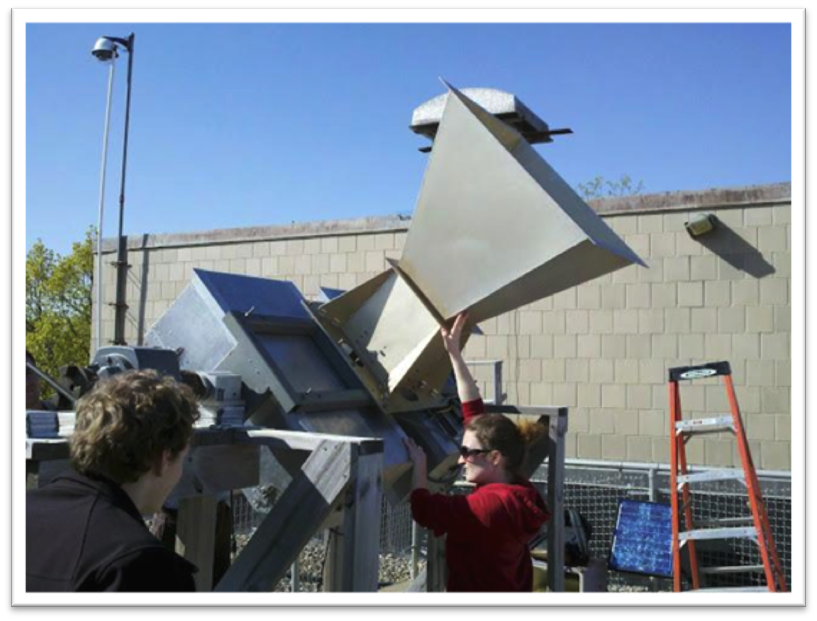
\includegraphics[width=0.4\linewidth]{images/agronomy_roof.png}
\end{figure}
\end{frame}

\begin{frame}
\begin{block}{Thesis Questions}
This thesis looks to explore the following questions: 
\begin{enumerate}
\item Can we use a SDR along with GNURadio to recreate a radiometer in software?
\item If so, what performance can we get from the system?
\item What benefits do we gain (if any) from using a SDR from a more traditional radiometer?
\end{enumerate}
The results of this research and experimentation are the subject of this thesis.
\end{block}

\end{frame}  


\subsection{Software Defined Radio} 

\subsection{GNURadio Software}

\subsection{Current ISU Radiometer}

\subsection{Related Works}

\section{General Theory of Operation}
\begin{frame}
\begin{block}{Radiometer}
The primary goal of a radiometer is to measure power.  While that statement sounds easy, there are in fact many factors that go in to how well a radiometer can measure the power it sees.  A better statement would be that a radiometer's primary goal is to accurately measure power within a certain degree of accuracy.  In order to accurately and within a high degree of precision measure power, a radiometer must take into account various factors such as the system noise, the bandwidth of the signal and the stability of the system as a whole. 
\end{block}
\end{frame}

\begin{frame}
\begin{block}{Measuring power}
To measure power in a radiometer, several factors are taken into consideration.  To begin with we have the noise signal coming from the antenna.  Our antenna is assumed to be looking at our target of interest and it is assumed that we can relate the antenna noise to the noise from the source.  It is often easier to refer to this noise as the brightness temperature.  Therefore the brightness temperature of the source can be related to the brightness temperature at the antenna.  We will refer to this brightness temperature as T$_{A}$.  

{\begin{figure}[h!tb] 
\centering
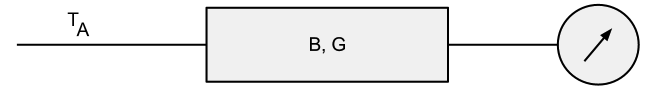
\includegraphics[width=\textwidth]{../Images/simple_rad.png}
\label{simplerad}
\end{figure}
}
\end{block}
\end{frame}

\begin{frame}
\begin{block}{Ideal Radiometer}
Figure on slide~\ref{simplerad} shows us an ideal radiometer.  That is a radiometer that has an input from the antenna, T$_{A}$, a known bandwidth denoted as B and a known gain denoted as G.  At the end of the block is the detector, which measures the power from the radiometer.
\end{block}
\end{frame}

\begin{frame}
\begin{block}{Bandwidth}
Only a certain selection of the radio spectrum is observed by the radiometer.  This is referred to as the bandwidth of the radiometer and is denoted as B or as $\beta$.  This bandwidth is then centered around a center frequency.  In our case, we center around 1.405 GHz as this falls in a protected frequency range often used for radiometry.  
\end{block}
\end{frame}

\begin{frame}
\begin{block}{Power}
The power coming from the antenna is amplified so it is easier to determine changes in the brightness temperature.  The overall gain of the radiometer system is referred to as G in this case.  Finally, we need to apply Boltzmann's constant, referred to as \textit{k}.  With these values, we can now compute the power the radiometer will see for an ideal radiometer.  This can be shown in equation~\ref{eq:power_rad_eq}

\begin{equation} \label{eq:power_rad_eq}
P=k*\beta*G*(T_{A})
\end{equation}
\end{block}

\end{frame}

\begin{frame}
\begin{block}{Noise}
However, since we do not have an ideal radiometer, we have another key component that needs to be addressed and that is the noise added to the system from the radiometer itself.  Most of the additional noise is from the Low Noise Amplifiers (LNA) that are used to increase the signal while attempting to keep the noise added to a minimum.  The Figure below shows the additional noise that is injected into the system.

{\begin{figure}[h!tb] 
\centering
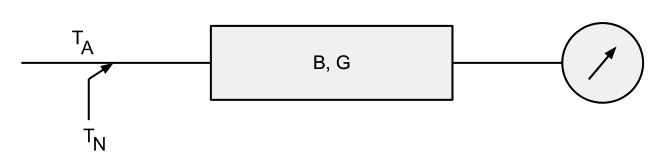
\includegraphics[width=\textwidth]{../Images/radiometer_noise_added.png}
\label{noiserad}
\end{figure}
}
\end{block}
\end{frame}

\begin{frame}
\begin{block}{Antenna Noise}
As it can be seen, this additional noise is added to the noise coming from the antenna source.  Therefore T$_{N}$ is added to T$_{A}$ and our final equation for the power measured is shown in equation~\ref{eq:final_power}.  

\begin{equation} \label{eq:final_power}
P=k*\beta*G*(T_{A}+T_{N})
\end{equation}
\end{block}
\end{frame}

\begin{frame}
\begin{block}{Sensitivity}
The ability of a radiometer to detect these small changes is the radiometer's sensitivity, or the standard deviation of the output signal from the radiometer.  This sensitivity is also referred to as the Noise Equivalent $\Delta$ Temperature or NE$\Delta$T. 

\begin{equation}
NE\Delta T=\frac{T_{A}+T_{N}}{\sqrt{\beta + \tau}}
\end{equation}
\end{block}
\end{frame}


\subsection{Software Defined Radios}
\begin{frame}
\begin{block}{SDR}
A software defined radio (SDR) attempts to mimic radio functions in software instead of relying on dedicated hardware.  A radiometer is a radio that can detect changes in power.  Therefore the SDR needs to be able to measure power coming from the source that we are looking at. 
\end{block}
\end{frame}

\begin{frame}
\begin{block}{Implementing a TPR}
The SDR is able to implement a total power radiometer, but in a slightly different way than a traditional radiometer.  A traditional radiometer will use a device called a square-law detector to measure the incoming RF signal power.  For the SDR, the incoming signal is sampled and converted to IQ values.  The IQ values represent the amplitude and phase information of the signal.  In GNURadio we are then able to square these values within software.  This block in GNURadio mathematically performs the following:

\begin{equation}
I^2+Q^2 = P_{out}
\end{equation}
\end{block}
\end{frame}

\begin{frame}
\begin{block}{IIR Filter}
This signal will fluctuate rapidly and to improve the sensitivity of the radiometer we wish to integrate this signal.  A RC filter is analogous to an integrator where the R and C values determine our time constant and our integration time for the filter.  A SDR however operates in the digital domain at discrete intervals.  One type of filter that can be used in the Infinite Impulse Response (IIR) filter. 
\end{block}
\end{frame}

\begin{frame}
\begin{block}{RC Filter}
To begin with, we look at what an analog RC filter looks like. 

{\begin{figure}[h!tb] 
\centering
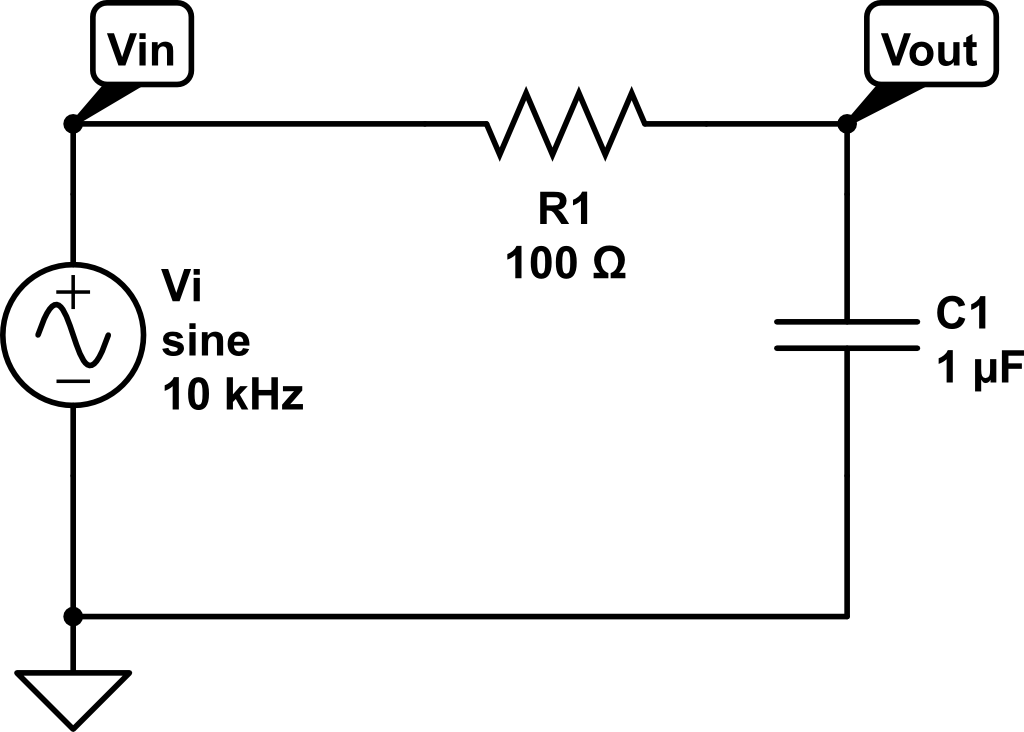
\includegraphics[width=7cm]{../Images/rc-circuit.png}
\label{rc_circuit}
\end{figure}
}
\end{block}
\end{frame}

\begin{frame}
\begin{block}{RC Filter Eqs}
This circuit can be represented by the following equation.
\begin{equation}\label{eq:rc_circuit_eq}
\frac{V_{in}-V_{out}}{R}=C\frac{dV_{out}}{dt}
\end{equation}
\end{block}
\end{frame}

\begin{frame}
\begin{block}{FIR Filter}
A Finite Impulse Response (FIR) filter is a digital filter that can take an impulse signal and decays to zero after a finite number of iterations.  This type of digital filter can be represented by the following equation:

\begin{equation}
y_n=\displaystyle\sum\limits_{i=o}^{P-1} c_ix_{n-i}
\end{equation}
\end{block}
\end{frame}

\begin{frame}
\begin{block}{IIR Filter}
An Infinite Impulse Response (IIR) filter is the same as the FIR filter, except that we add an additional summation term which feeds back the previous output.

\begin{equation}
y_n=\displaystyle\sum\limits_{i=o}^{P-1} c_ix_{n-i}+\displaystyle\sum\limits_{j=1}^{Q} d_jy_{n-j}
\end{equation}

It can be seen that a FIR filter is really a IIR filter except that $Q=0$.  
\end{block}
\end{frame}

\begin{frame}
\begin{block}{IIR and RC Filter}
To get a better understanding on how our digital IIR filter relates to our RC filter analog, we can look at the Fourier Transform and the relationship of the input to the output in the frequency domain.

\begin{equation}
H(f)=\frac{\displaystyle\sum\limits_{j=o}^{P-1} c_je^{-2\pi ijfT}}{1-\displaystyle\sum\limits_{k=1}^{Q} d_ke^{-2\pi ikfT}}
\end{equation}

Here $f$ is our frequency in Hz and $T$ is the time between samples in seconds.
\end{block}
\end{frame}

\begin{frame}
\begin{block}{Link between RC and IIR}
We now want show the link between our analog RC circuit and the IIR filter.  Looking at equation \ref{eq:rc_circuit_eq}, which represents the differential equation relating the input voltage $V_{in}$ to the output voltage $V_{out}$, we can substitute for input and output of our IIR filter.  Since we are now in the time domain, we need to define what $T$ is.

\begin{equation}
T=time between samples=\frac{1}{sampling rate}
\end{equation}
\end{block}
\end{frame}

\begin{frame}
\begin{block}{input voltage to IIR}
We can now relate our input voltage to the input to our IIR filter and the output voltage to the output of our IIR filter.

\begin{equation}
x_n=v_{in}(nT)
\end{equation}

\begin{equation}
y_n=v_{out}(nT)
\end{equation}
\end{block}
\end{frame}

\begin{frame}
\begin{block}{Rewrite difference eq}
We can now rewrite our difference equation with $x_n$ and $y_n$.

\begin{equation}
\frac{x_n-y_n}{R}=C\frac{y_n-y_{n-1}}{T}
\end{equation}

Now, we can solve for $y_n$ which results in our final equation for showing how a IIR filter is related to an RC filter.

\begin{equation}
y_n=\frac{T}{T+RC}x_n+\frac{RC}{T+RC}y_{n-1}
\end{equation}
\end{block}
\end{frame}

\begin{frame}
\begin{block}{IIR and RC filter}
It can be seen that an IIR filter can have the same frequency response as we would expect from an analog RC filter.  As our sampling rate approaches infinity, the approximation gets closer to the original response from the analog RC circuit.  

\end{block}
\end{frame}
\subsection{GNURadio Software}

\subsection{RF Front End}

\section{GNURadio and N200 TPR}

\subsection{Hardware}

\subsubsection{Requirements}

\subsubsection{Noise Temperature Considerations}

\subsubsection{Existing ISU Radiometer RF Front End}

\subsection{Software}

\subsubsection{Requirements}

\subsubsection{Obtaining Signal Information and GUI Controls}

\subsubsection{Implantation of a TPR in Software}

\subsubsection{Data Storage and Display}

\section{Testing and Verification}

\subsection{Square-law Detector}

\subsection{SDR Tests}

\subsection{E E 518 Lab Tests}

\subsection{LN2 Tests}

\section{Performance and Evaluation}

\subsection{Sensitivity, Accuracy and Stability}

\subsection{Required Performance}

\subsection{Square-law Detector Performance}

\subsection{SDR Performance}

\section{Conclusion and Future Work}


\begin{frame}
\frametitle{Bullet Points}
\begin{itemize}
\item Lorem ipsum dolor sit amet, consectetur adipiscing elit
\item Aliquam blandit faucibus nisi, sit amet dapibus enim tempus eu
\item Nulla commodo, erat quis gravida posuere, elit lacus lobortis est, quis porttitor odio mauris at libero
\item Nam cursus est eget velit posuere pellentesque
\item Vestibulum faucibus velit a augue condimentum quis convallis nulla gravida
\end{itemize}
\end{frame}


\begin{frame}
\frametitle{Multiple Columns}
\begin{columns}[c] % The "c" option specifies centered vertical alignment while the "t" option is used for top vertical alignment

\column{.45\textwidth} % Left column and width
\textbf{Heading}
\begin{enumerate}
\item Statement
\item Explanation
\item Example
\end{enumerate}

\column{.5\textwidth} % Right column and width
Lorem ipsum dolor sit amet, consectetur adipiscing elit. Integer lectus nisl, ultricies in feugiat rutrum, porttitor sit amet augue. Aliquam ut tortor mauris. Sed volutpat ante purus, quis accumsan dolor.

\end{columns}
\end{frame}

%------------------------------------------------
\section{Second Section}
%------------------------------------------------

\begin{frame}
\frametitle{Table}
\begin{table}
\begin{tabular}{l l l}
\toprule
\textbf{Treatments} & \textbf{Response 1} & \textbf{Response 2}\\
\midrule
Treatment 1 & 0.0003262 & 0.562 \\
Treatment 2 & 0.0015681 & 0.910 \\
Treatment 3 & 0.0009271 & 0.296 \\
\bottomrule
\end{tabular}
\caption{Table caption}
\end{table}
\end{frame}

%------------------------------------------------

\begin{frame}
\frametitle{Theorem}
\begin{theorem}[Mass--energy equivalence]
$E = mc^2$
\end{theorem}
\end{frame}

%------------------------------------------------

\begin{frame}[fragile] % Need to use the fragile option when verbatim is used in the slide
\frametitle{Verbatim}
\begin{example}[Theorem Slide Code]
\begin{verbatim}
\begin{frame}
\frametitle{Theorem}
\begin{theorem}[Mass--energy equivalence]
$E = mc^2$
\end{theorem}
\end{frame}\end{verbatim}
\end{example}
\end{frame}

%------------------------------------------------

\begin{frame}
\frametitle{Figure}
Uncomment the code on this slide to include your own image from the same directory as the template .TeX file.
%\begin{figure}
%\includegraphics[width=0.8\linewidth]{test}
%\end{figure}
\end{frame}

%------------------------------------------------

\begin{frame}[fragile] % Need to use the fragile option when verbatim is used in the slide
\frametitle{Citation}
An example of the \verb|\cite| command to cite within the presentation:\\~

This statement requires citation \cite{p1}.
\end{frame}

%------------------------------------------------

\begin{frame}
\frametitle{References}
\footnotesize{
\begin{thebibliography}{99} % Beamer does not support BibTeX so references must be inserted manually as below
\bibitem[Smith, 2012]{p1} John Smith (2012)
\newblock Title of the publication
\newblock \emph{Journal Name} 12(3), 45 -- 678.
\end{thebibliography}
}
\end{frame}

%------------------------------------------------

\begin{frame}
\Huge{\centerline{The End}}
\end{frame}

%----------------------------------------------------------------------------------------

\end{document} 